\chapter{Results}

The results will include three parts. 
First, the performance of rCOMMIT will be visualized from different angles. Second, the performance of the models based on the 
pseudo ground truth will be shown. Last, a comparison between the results from COMMIT and SIFT is conducted.

\section{Performance of rCOMMIT}

Fig \ref{fig:heatmap} shows the distribution of AR ranges in different subset sizes on three subjects. 

\begin{figure}[ht]
    \centering
    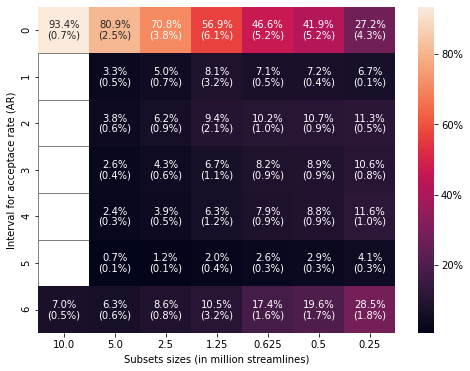
\includegraphics[width= 15cm]{figures/heatmap.png}
        \caption{The 
        }
    \label{fig:heatmap}
\end{figure}

\subsection{Pseudo Ground Truth}

\section{Model Classification}

\section{Comparison Between COMMIT and SIFT}

\subsection{Performance between methods}








Describe the results of the degree project.
